% \documentclass[12pt]{article}

%%v helpful MIT exam schema, see http://www-math.mit.edu/~psh/exam/examdoc.pdf
 \documentclass[9pt]{exam} 
% \qformat{\textbf{Question \thequestion}\quad \thepoints\hfill } % Large depth to make space}
 \renewcommand{\thesubpart}{(\roman{subpart})}
 \renewcommand{\subpartlabel}{\thesubpart}
 \footer{}{}{Page \thepage\ de \numpages}
\addpoints
\pointsinmargin
%\boxedpoints
\renewcommand{\questionshook}{\setlength{\itemsep}{2mm}}
\renewcommand{\partshook}{
	\setlength{\itemsep}{0.5cm}
%   	\setlength{\leftmargin}{-10pt}%
}

\usepackage{cmbright}

\pagestyle{empty} %for handouts
\addtolength{\jot}{2em} % this makes all formulae a bit more spaced vertically for handouts
\setlength{\parindent}{0pt} %we're not writing a novel
%\renewcommand{\arraystretch}{2} %makes tables taller, so easier to write in

\usepackage[fleqn]{amsmath}
\usepackage{amssymb} %standard classy maths symbols
\usepackage[a4paper, margin=1in]{geometry} %makes it easy to specify where to put stuff on the page

\usepackage{siunitx} %v handy way of getting SI units to typeset correctly...
% \sisetup{locale = FR} %... and now it will use a comma for decimals

\usepackage[utf8]{inputenc}

% \usepackage[french]{babel} % frenchify everything (e.g. a Table becomes a Tableau)
% \usepackage{lmodern} % font with nicer French characters than standard
\usepackage{textcomp} % and more help for special characters

\usepackage{tcolorbox} % basic but good package for boxes around text
\tcbset{colback=black!5!white}
% \usepackage{color} % colours
%\newcommand{\fillin}{\color{black!1!white}} %makes the text disappear
%\definecolor{fillin}{rgb} {1.00,1.00,1.00}
%\renewcommand{\fillin}{\color{blue}} \definecolor{fillin}{rgb} {0.00,0.00,1.00} %makes the filling in text appear (in blue)

%\usepackage{enumitem} % can change the labels on lists, items, enumerates

\usepackage{tikz, pgfplots} % interval diagrams, sets, etc.
\usetikzlibrary{calc,trees,positioning,arrows,fit,shapes}

\begin{document}

\textbf{Name:} \dotfill

\

\begin{questions}

\question[1] Put these five steps into the correct order for solving a trigonometry problem.

\begin{center}
\textbf{State} the trig ratio \hspace{10mm}
\textbf{Solve} the equation \hspace{10mm}
\textbf{Sketch} the triangle

\textbf{Name} the sides (hyp, opp, adj) \hspace{10mm}
\textbf{Subsitute}

\emph{En français : énoncer, résoudre, esquisser, nommer et substituter.}
\end{center} 

\fillwithdottedlines{10mm}

\question[4] Find the length $x$. \emph{No need to sketch a new triangle.}

\

\begin{minipage}{0.4\textwidth}
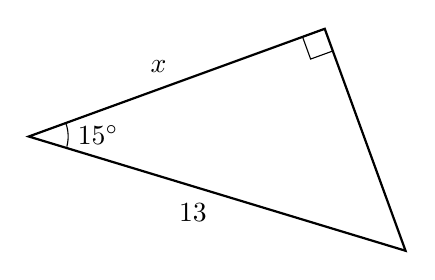
\begin{tikzpicture}[scale = 1, rotate = 200]
\draw[thick] (0, 0) -- node[above left] {$x$} (4, 0) -- node[below left]{$13$} (0, 3) -- cycle;
\draw (0, 0) rectangle ++(0.3, 0.3);
\draw (3.5, 0) arc (180:145:0.5) node[pos=0.5, right] {$15^\circ$};
\end{tikzpicture}
\end{minipage}
\begin{minipage}{0.55\textwidth}
\fillwithdottedlines{45mm}
\end{minipage}

\

\question[5]  Since 2008 the highest building ever constructed is the skyscraper \emph{"Burj Khalifa"} in Dubaï. At a distance of \SI{1,7}{km} from the base, the top makes an angle of 26° with the horizon. 

Calculate its height to the nearest metre. \emph{Careful with the units!}



\vfill

\question[0] \textbf{Bonus.} Calculate $\,\,(\sin \theta)^2 + (\cos \theta)^2\,\,$ for $\theta \in \{ 10^\circ; \, 20^\circ; \, 30^\circ; \ldots \}$. What can you say?

\end{questions}

\begin{tcolorbox}

\textbf{Name of marker:}

\begin{center}
\gradetable[h][questions]
\end{center}

\end{tcolorbox}


\end{document}